\section{Using Partial Orders}

\begin{figure}
	\centering
	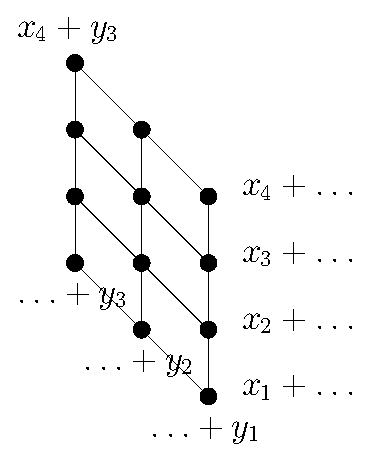
\includegraphics[height=0.2\textheight]{fig/open/x+y}
	\caption{Typical Hasse diagram for the Sorting $X + Y$ problem.}
	\label{fig:xy:poset:chains}
\end{figure}

\begin{figure}
	\centering
	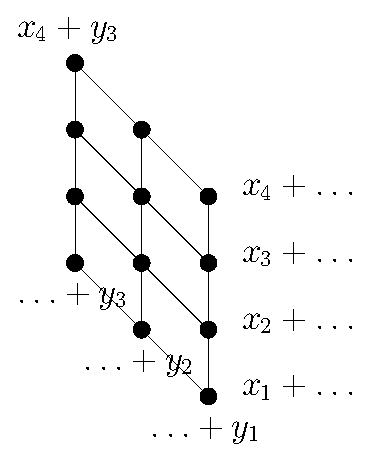
\includegraphics[height=0.2\textheight]{fig/open/x+y}
	\caption{Typical Hasse diagram for the Sorting $X + Y$ problem.}
	\label{fig:xy:poset:antichains}
\end{figure}

\begin{figure}
	\centering
	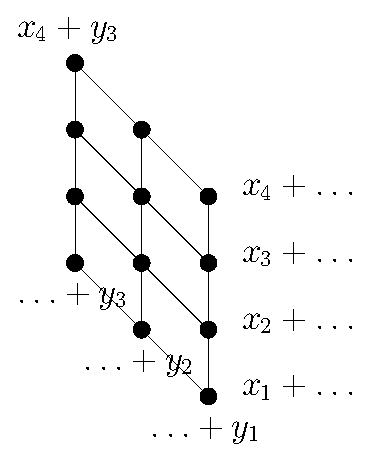
\includegraphics[height=0.2\textheight]{fig/open/x+y}
	\caption{Typical Hasse diagram for the Sorting $X + Y$ problem.}
	\label{fig:xy:poset:compgraph}
\end{figure}

\begin{figure}
	\centering
	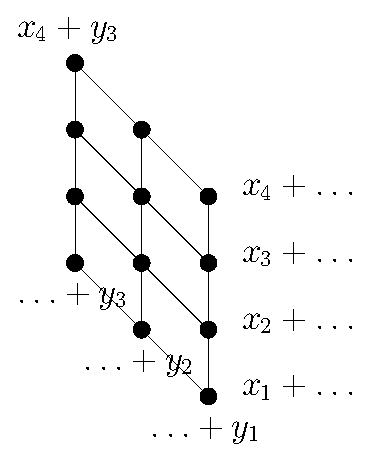
\includegraphics[height=0.2\textheight]{fig/open/x+y}
	\caption{Typical Hasse diagram for the Sorting $X + Y$ problem.}
	\label{fig:xy:poset:incompgraph}
\end{figure}

\begin{figure}
	\centering
	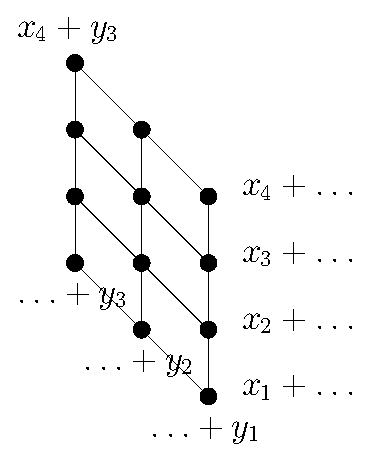
\includegraphics[height=0.2\textheight]{fig/open/x+y}
	\caption{Typical Hasse diagram for the Sorting $X + Y$ problem.}
	\label{fig:xy:poset:mergesort}
\end{figure}

\begin{figure}
	\centering
	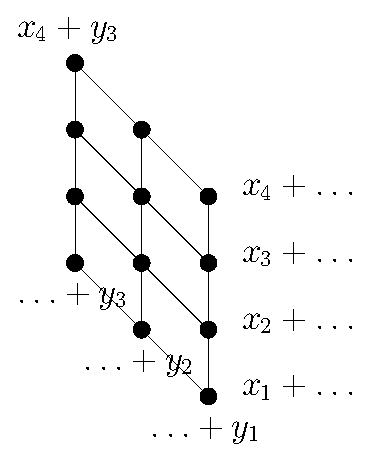
\includegraphics[height=0.2\textheight]{fig/open/x+y}
	\caption{Typical Hasse diagram for the Sorting $X + Y$ problem.}
	\label{fig:xy:poset:mergexy}
\end{figure}


In this first attempt we will use the partial order structure of the order on
the elements in $X + Y$.

\ref{fig:open:xy} shows us all the order relations between elements of $X + Y$.
There are chains and antichains according to a regular pattern, we highlight
them in \ref{fig:xy:poset:chains} and \ref{fig:xy:poset:antichains}. In
\ref{fig:xy:poset:compgraph} and \ref{fig:xy:poset:incompgraph} we show the
comparability and incomparability graphs of the problem.

Now we will solve this problem in a strictly faster way than sorting all
of its elements, by taking advantage of some of the information we already have.

First, note that sorting $X + Y$ without information using the merge sort
algorithm would use $2 n^2 \log n$ comparisons. We will show that it is
possible to sort $X + Y$ with half the comparisons.

The merge sort algorithm has this particularity that at the end of every step
of the recursion we are left with several total orders on disjoint subsets of
the set to sort. To illustrate, if we organise steps in stages we obtain what
is shown in \ref{fig:xy:poset:mergesort}.

Now, if we highlight a specific subset of disjoint chains of our Hasse diagram,
we obtain the picture shown in \ref{fig:xy:poset:mergexy}. This figure
clearly, depicts one of the stages in the resolution of the merge sort recursion.

Remember that in merge sort there are $\log N$ stages. At stage $i$ we have
built $2^{i}$ total orders on disjoint subsets of size $2^{\log N - i}$. Since
the stage represented in \ref{fig:xy:poset:mergexy} shows $n$ total orders on
disjoint subsets of size $n$, and that the total number of elements in $X+Y$ is
$N = n^2$ we can conclude that \ref{fig:xy:poset:mergexy} shows us step
$\sfrac{1}{2} \log N$. In merge sort, at each stage of the recursion we do at
most N comparisons hence we only have half of the comparisons left to do in
order to complete the execution of the algorithm.


